%% LaTeX2e class for student theses
%%
%% Karlsruhe Institute of Technology
%% Institute of Information Security and Dependability
%% Software Design and Quality (SDQ)
%%
%% Dr.-Ing. Erik Burger
%% burger@kit.edu
%%
%% Version 1.6, 2024-06-07

\chapter{Implementation}
\label{ch:Implementation}

This chapter describes the implementation of the proposed features to the \LiSSAf to optimize classification prompts for fixed datasets.
To achieve this goal, a new \promptoptimizer module is added to the \LiSSA pipeline.
This module can be combined with further optional \metric and \evaluator modules to enable a flexible and reusable architecture.
\autoref{fig:component_diagramm} provides an overview of the components involved in this implementation.

\begin{figure}
    \centering
    \includegraphics[width=\textwidth]{graphics/class_diagrams/components}
    \caption{Overview of the major new components involved in the implementation}
    \label{fig:component_diagramm}
\end{figure}

\section{Prompt Optimizer Module}
\label{sec:impl:prompt_optimizer_module}

The prompt optimizer module provides implementations for the actual prompt optimization.
The only method this module is required to implement is the \method{optimize} \Todo{Check if this method is still named the same} method.
It requires the source and target \elementstore created in the previous pipeline steps.
They contain the artifacts to be linked.
The module will be instantiated with a set of configuration parameters, again following the format of the \LiSSAf.
A factory class is used to create the module based on the configuration.
Furthermore, the \metric and \evaluator modules are provided to the respective constructors if required.

\begin{figure}
    \centering
    \fontsize{8}{10}\selectfont
    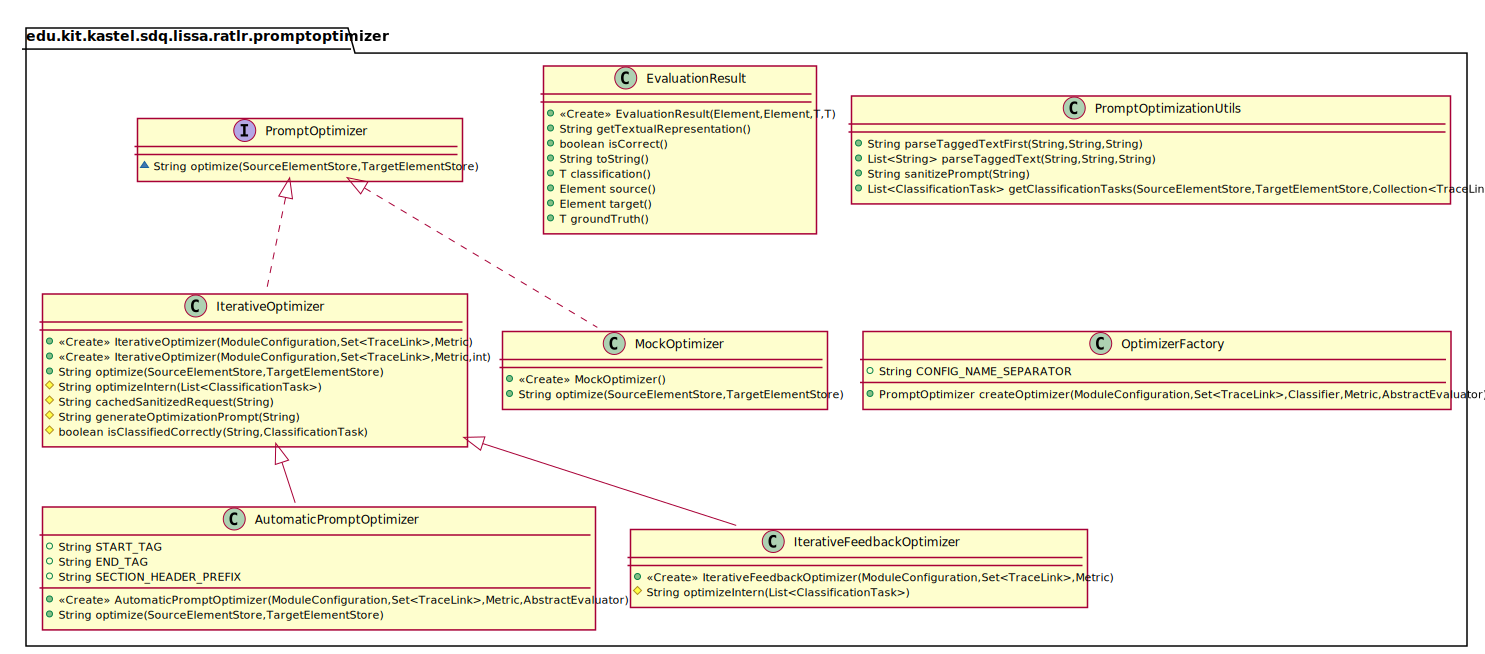
\includegraphics[width=\textwidth]{graphics/class_diagrams/optimizer}
    \caption{The new \promptoptimizer module and its implementations}
    \label{fig:optimizer_module_diagramm}
\end{figure}

As seen in \autoref{fig:optimizer_module_diagramm}, the \promptoptimizer module will typically use the \LLM to evaluate different prompts.
\Todo{It has not been seen...}

Many implementations of the \promptoptimizer module will require sampling strategies as a heuristic to reduce the number of calls to the \LLM.
\Todo{Is heuristic the right word here?}
The \samplingstrategy submodule provides different strategies to select a sublist of comparable elements from a collection.
The strategies can be instantiated with configuration parameters and are used by the \promptoptimizer module.
This way, sampling strategies can be swapped easily without changing the actual optimization logic.
The random sampler uses a fixed random seed to ensure reproducibility of results.

\begin{figure}
    \centering
    \fontsize{8}{10}\selectfont
    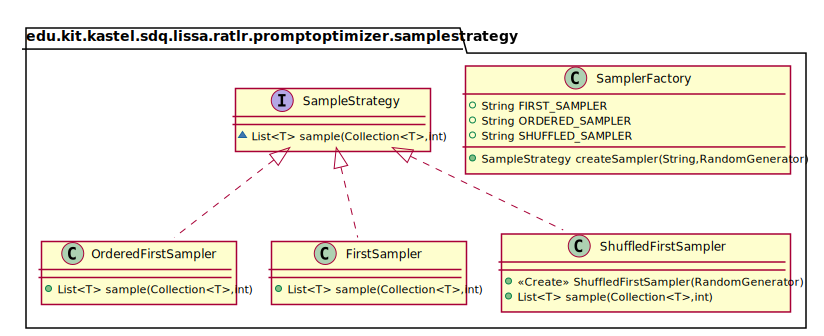
\includegraphics[width=\textwidth]{graphics/class_diagrams/sample_strategy}
    \caption{The new \samplingstrategy submodule and its implementations}
    \label{fig:sampling_strategy_diagramm}
\end{figure}

In \autoref{fig:sampling_strategy_diagramm}, the sampling strategy submodule is depicted.
Currently, three different strategies are implemented.
\begin{itemize}
    \item The \method{ShuffledFirstSampler} will shuffle the input list using the \method{RandomGenerator} and return the first elements.
    \item The \method{OrderedFirstSampler} will sort the input list and return the first elements.
    \item The \method{FirstSampler} will return the first elements of the input list.
\end{itemize}

\section{Metric Module}
\label{sec:impl:metric_module}
The \metric component provides implementations for different metrics to score the quality of a prompt on a given set of tasks.
Metrics can be divided into two major categories.
Pointwise metrics will evaluate each \TL prediction and return a separate score for each.
Scoring strategies for pointwise metrics are provided by the \scorer submodule.
The overall score can then be calculated by reducing the individual scores using a \reductor.
The \reductor submodule provides different strategies to reduce a collection of scores to a single value.
In contrast, global metrics will evaluate the entire set of \TL predictions at once and return a single score directly.
This is because they factor in relationships between different predictions, like whether the correct prediction is a true positive or a true negative.

The scores are cached using \LiSSAs built-in \cache module.

\begin{figure}
    \centering
    \fontsize{8}{10}\selectfont
    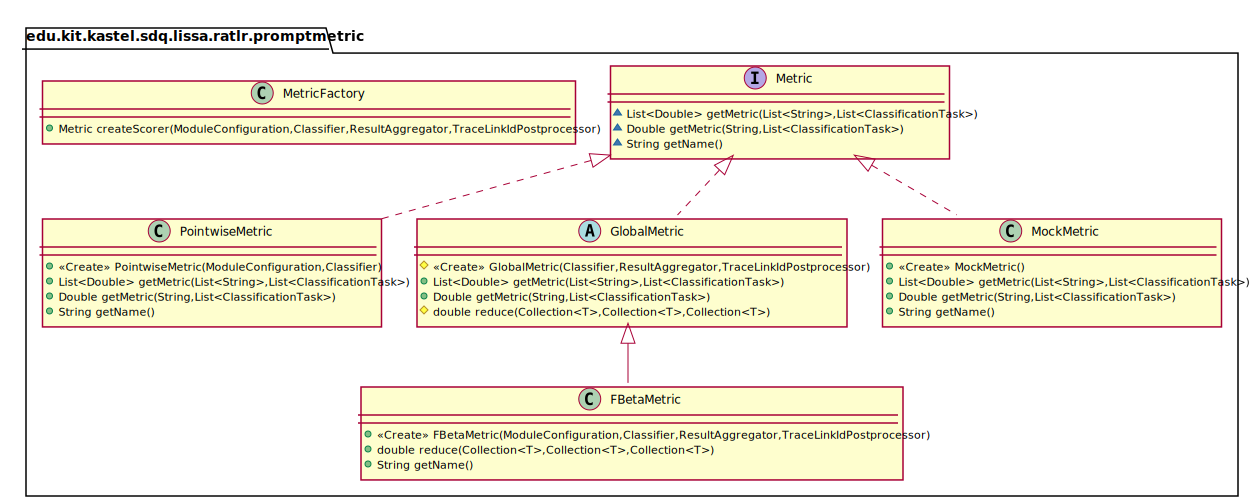
\includegraphics[width=\textwidth]{graphics/class_diagrams/metric}
    \caption{The new \metric module and its implementations}
    \label{fig:metric_module_diagramm}
\end{figure}

Currently, only the \fbeta metric is implemented as a global metric.
The beta parameter can be altered in the module configuration.
The pointwise metric implementation relies on the \method{Binary}\scorer and the \method{Mean}\reductor.
This is also portrayed in \autoref{fig:scorer_reductor_diagramm}.
The \method{Binary}\scorer will return a score of 1.0 for a correct prediction and 0.0 otherwise.
A correct prediction is defined as predicting a \TL for a pair of artifacts that actually has a \TL in the ground truth or not predicting a \TL for a pair of artifacts that does not have a \TL in the ground truth.
The \method{Mean}\reductor will then compute the mean of all individual scores to return a single value.


\begin{figure}
    \centering
    \fontsize{8}{10}\selectfont
    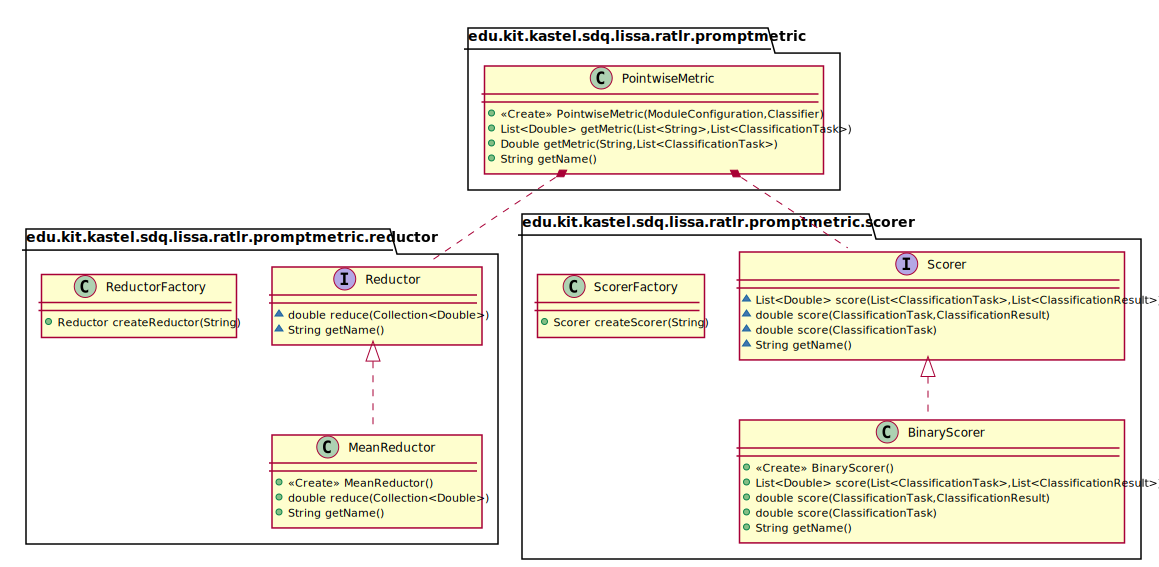
\includegraphics[width=\textwidth]{graphics/class_diagrams/pointwise_metric}
    \caption{The submodules utilized by the pointwise metric implementation}
    \label{fig:scorer_reductor_diagramm}
\end{figure}

\section{Evaluator Module}
\label{sec:impl:evaluator_module}
The \evaluator module provides implementations to evaluate the quality of a prompt on a given set of tasks.
In contrast to the \metric module, the \evaluator will not use all tasks to compute the prompt score.
Instead, more complex sampling strategies can be used to select a subset of tasks.
This is especially useful for larger datasets, where evaluating all tasks would be too costly.
The \ucb bandit evaluator is the most noteworthy implementation.
It will use the \ucb algorithm to select a subset of tasks that are expected to provide the most information gain.
This is achieved by balancing exploration and exploitation.
The size of the subset can be configured in the module configuration.
The \ucb evaluator can be configured with a random seed to ensure reproducibility of results.

\begin{figure}
    \centering
    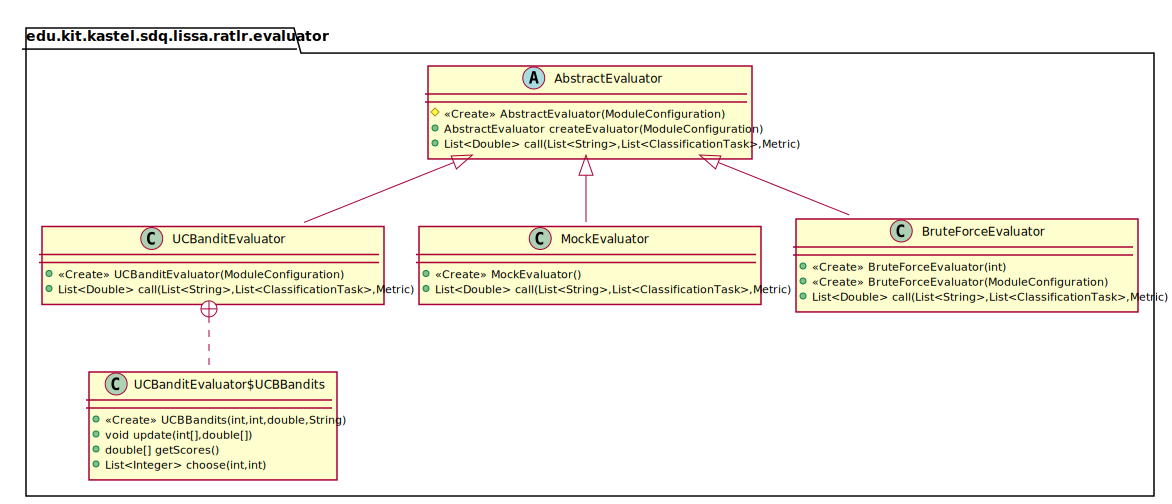
\includegraphics[width=\textwidth]{graphics/class_diagrams/evaluator}
    \caption{The new \evaluator module and its implementations}
    \label{fig:evaluator_module_diagramm}
\end{figure}

Other implementations seen in \autoref{fig:evaluator_module_diagramm} are the \method{BruteForceEvaluator}, which will use all tasks to evaluate the prompt.
The \method{MockEvaluator} is used for testing purposes and will return a fixed score.

\section{LiSSA Pipeline Integration}
\label{sec:impl:lissa_integration}
\Todo{Can you use \acs{LiSSA} in the title but without the quote?}
The new modules are integrated into the \LiSSA pipeline.
A new command was added to the \LiSSA command-line interface to run the prompt optimization.
The command will read the configuration file and create the required modules using their constructors or factories, respectively.
While the optimization pipeline, as a standalone, is independent of the regular evaluation pipeline, they can be combined.
This is achieved by feeding the optimized prompt from the optimization pipeline into the evaluation pipeline, indicated by a separate configuration.
